\documentclass[12pt]{article}
\usepackage[top=1in, bottom=1in, left=1in, right=1in]{geometry}
\usepackage{graphicx}
\linespread{2}

\newcommand{\p}{\textit{Paramecium}}

\begin{document}
\title{The Effects of $\mathrm{KCl}$ on \textit{Paramecium caudatum} Motion}
\author{Samuel Deslandes}
\date{\today}
\maketitle

\section{Introduction}
	\textit{Paramecium caudatum} is a species of unicellular organism from the phylum Ciliophora. As a ciliate, \p\ move using hair-like organelles which surround the outer surface of the cell called cilia. These cilia act as paddles, which move in a coordinated wave of whiplash motions to propel the \p\ through its environment.     
\section{Design}

\section{Results}
	Test text Test text Test text Test text Test text Test text Test text Test text Test text Test text Test text Test text Test text Test text Test text Test text Test text Test text Test text Test text Test text Test text Test text Test text Test text Test text Test text Test text Test text Test text Test text Test text Test text Test text Test text Test text Test text Test text Test text Test text Test text Test text Test text Test text Test text Test text Test text Test text Test text Test text Test text Test text 
	
	\begin{figure}[h]
		\centering
		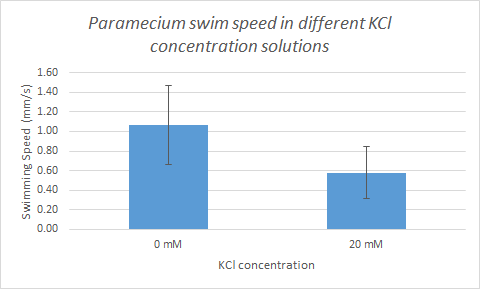
\includegraphics{chart1.png}
		\caption{Mean swimming speeds of the \p\ in 0 and 20 mM KCl concentration solutions. Error bars represent standard deviation.}
		\label{barGraph}
	\end{figure} 
	
\section{Discussion}

\section{Conclusion}

\end{document}